\originalsection{作业 8: 势能与守恒}
\begin{exercise}
原题 1. 质量 $m$ 块把弹簧 $k$ 压缩 $x$ 后释放, 沿光滑轨道进入半径 $R$ 的竖直环. 到环顶时法向力为重力的两倍. 求 $x$.
\end{exercise}
\begin{solution}
环顶向心方程 $2mg+mg=mv_t^2/R$, $v_t^2=3gR$. 从底部弹簧储能到顶点守恒: $kx^2/2=2mgR+mv_t^2/2=7mgR/2$. 因而 $x=\sqrt{7mgR/k}$.
\end{solution}
\begin{exercise}
原题 2. 质量 $m$ 球由长 $l$ 绳悬挂, 在底点被击后速率 $v_0$, 作竖直圆周运动. (a) 环顶张力多少? (b) 环顶时脱离绳, 回到环底高度时距底点水平距离 $d$ 多少? 忽略阻力.
\end{exercise}
\begin{solution}
上升高度 $2l$, $v_t^2=v_0^2-4gl$. (a) $T=m(v_t^2/l-g)=mv_0^2/l-5mg$, 完成绷紧圆周需 $v_0^2\ge5gl$. (b) 脱离时水平速度 $v_t$, 自由落下 $2l$ 用时 $2\sqrt{l/g}$, 所以 $d=2\sqrt{(l/g)(v_0^2-4gl)}$.
\end{solution}
\begin{exercise}
原题 3. 竖直光滑环半径 $R$. 重物 $3m$ 连劲度系数 $k$、自然长为零的理想弹簧, 弹簧锚点在环心左方 $2R$ 处. 轻物 $m$ 静止在环底. 重物从环顶静止释放, 在环底与轻物粘合. 求刚能到达环最右点 A (与圆心等高) 而不再升高的 $m$.
\end{exercise}
\begin{solution}
环顶和底的弹簧长度均为 $\sqrt5R$, 第一次下降释放 $6mgR$, 故碰前 $v_-^2=4gR$. 碰后 $v_+=3v_-/4$, 动能为 $9mgR/2$. 从底到 A, 重力势能增 $4mgR$, 弹簧长从 $\sqrt5R$ 到 $3R$, 势能增 $2kR^2$. 等式 $9mgR/2=4mgR+2kR^2$ 给 $m=4kR/g$. 对此质量底到 A 的总势能单调增加, 所以没有更早转向点.
\end{solution}
\begin{exercise}
原题 4. 发射物质量 $m$ 从地球表面以逃逸速度竖直射出. 地球半径 $R_e$、质量 $m_e$. 到地心距 $2R_e$ 时, 与同质量的圆轨道卫星正交碰撞并粘合. (a) 初速. (b) 碰前发射物速率. (c) 碰前卫星速率. (d) 合体碰后速率.
\end{exercise}
\begin{solution}
(a) $v_0=\sqrt{2Gm_e/R_e}$. 发射物总能量为零, 所以 (b) $v_p=\sqrt{Gm_e/R_e}$. (c) 圆轨道 $v_s=\sqrt{Gm_e/(2R_e)}$. (d) 速度向量正交, 由动量守恒合体速率为 $\sqrt{v_p^2+v_s^2}/2=\sqrt{3Gm_e/(8R_e)}$. 此后轨道一般不是圆.
\end{solution}
\begin{exercise}
原题 5. 一维势能 $U(x)=-U_0e^{-x^2/a^2}$, $U_0,a>0$. (a) 画势能图, 选 $-U_0<E<0$ 并标一位置的动能、势能与总能量. (b) 求力. (c) 求原点速率使转向点恰为 $x=\pm a$.
\end{exercise}
\begin{solution}
(a) 势阱在原点最低 $-U_0$, 两端趋零. 以下取 $E=-U_0/2$, 所标竖线给 $K=E-U$. (b) $F=-2U_0x e^{-x^2/a^2}/a^2$. (c) $E=U(a)=-U_0/e$, 故 $v(0)=\sqrt{2U_0(1-e^{-1})/m}$.
\begin{center}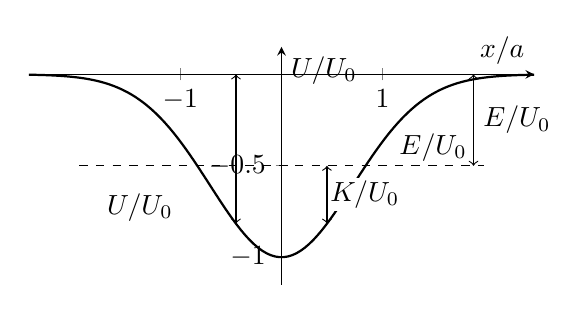
\begin{tikzpicture}
\begin{axis}[width=8cm,height=4.6cm,axis lines=middle,clip=false,xlabel={$x/a$},ylabel={$U/U_0$},xmin=-2.5,xmax=2.5,ymin=-1.15,ymax=.15,xtick={-1,0,1},ytick={-1,-.5},samples=120]
\addplot[thick,domain=-2.5:2.5]{-exp(-x*x)};
\addplot[dashed,domain=-2:2]{-.5};\node at(axis cs:1.5,-.4){$E/U_0$};
\draw[<->](axis cs:.45,-.81669)--(axis cs:.45,-.5) node[midway,right,fill=white,inner sep=1pt]{$K/U_0$};
\draw[<->](axis cs:-.45,0)--(axis cs:-.45,-.81669);
\node at(axis cs:-1.4,-.73){$U/U_0$};
\draw[<->](axis cs:1.9,0)--(axis cs:1.9,-.5) node[midway,right]{$E/U_0$};
\end{axis}\end{tikzpicture}\end{center}
\end{solution}
